\chapter{Lexicon}
\label{sec:LEX-lexicon}


% 
% The intended audience of the dictionary 
% 
% 
% Words from Ducie + usage english value
%  gives Chakali word not used in not Ducie



\section{Organisation and content}
\label{sec:LEX-Intro}
 
This section offers a Chakali-English dictionary and an English-Chakali index. 
The information they contain is extracted  from a database which I
started at the very beginning of the project.  At the  macro-structure level,
the database follows the Standard Format Marker (SFM),  which is a notational
standard implemented in the Summer Institute of Linguistics (SIL)' program
Shoebox/Toolbox.\footnote{http://www.sil.org/computing/toolbox/}   The SFM
database format is fixed, but has no predefined fields. However,  a  standard
consisting of a wide range of  lexicographic features has been developed by users 
over  the years. These lexicographic features, called {\it SFM fields}, 
may be interpreted by the Multi-Dictionary Formatter (MDF), which is a special
formatted output facility for dictionaries \citep[see][]{Cowa00}.  At the
micro-structure, the present dictionary and index are made out of  only a
selection of SFM fields and values which have been processed in and exported  
by 
Lexique
Pro.\footnote{http://www.lexiquepro.com/}    


\subsection{Chakali-English dictionary}

The Chakali-English dictionary consists of  2140 Chakali headword
entries.\footnote{29/10/10 version}  The headwords  are
alphabetically organized although an
arbitrary decision was taken to insert the letter `dʒ' after `d', `gb' after `g', `kp'
after `k',  `ɲ'  and `ŋm' successively after `n',  and `tʃ' after `t'.  
 The orthography is based on the  symbols used in the phonology outline of
chapter \ref{sec:chap-phono}, that is,  a Latin
alphabet supplemented with
symbols
from the International Phonetic Alphabet.  For  users accustomed to the literacy
work of
the Ghana Institute
of Linguistics, Literacy and Bible translation (GILLBT)\footnote{Reference is
made to the work of Marjorie Crouch\dag, Patricia Herbert, Noah Ampen, Kofi
Mensah, Mike Toupin, Vicky Toupin, Ian Gray and Claire Gray.} I provide a
correspondence table which identifies the differences between their
transcriptions and mine. The transcription adopted in the database  appears to
the right of the arrows. 

\begin{center} 
\framebox[3in]{
\begin{tabular}{lllllll}

ng &$\leftarrow$& ŋ  & \hspace*{5ex} y&$\leftarrow$& j\\
ny &$\leftarrow$& ɲ  &\hspace*{5ex} Vh&$\leftarrow$& Ṽ \\
ch  &$\leftarrow$& tʃ  &\hspace*{5ex}  i&$\leftarrow$&ɪ\\
j &$\leftarrow$&dʒ  &\hspace*{5ex}  u&$\leftarrow$& ʊ \\

\end{tabular}  
}
\end{center}

 
In (\ref{ex:LEX-cli-eng-entry}), two representative entries
of the Chakali-English dictionary are presented.\footnote{The circled numbers
in (\ref{ex:LEX-cli-eng-entry})  and (\ref{ex:LEX-index}) are there for
reference purposes only.}



\begin{exe}
\ex\label{ex:LEX-cli-eng-entry}
\begin{xlist}
\ex
\ding{192}{\B fi} 	\ding{193}[fí] \ding{194} {\it num}. \ding{196}ten.

\ex
\ding{192}{\B boro} \ding{193}[bòró] \ding{194}{\it n}. \ding{195}1 •
\ding{196}portion. \ding{197}{\B ma kpa a bar boro a tɪɛ ba} \ding{198}You gave
them some portion (of land). \ding{195}2 • short. \ding{197}{\B a baboroso
hama} \ding{198}Those short men over there.
\end{xlist}
\end{exe}

An entry starts with a  headword (\ding{192}), which is immediately followed by its
phonetic representation (\ding{193}). This
representation adds tones and other information on the pronunciation. Words
which do not bear tones in the phonetic representation field are considered
either toneless or  unresolved.  The part of speech
(\ding{194}) provides  the morphosyntactic category of the
headword. Meaning is represented in the following way: if the headword has more
than one sense,  a number followed by a black
dot
(\ding{195}) enumerates the different senses. Slight differences are
separated by a comma within the same field.  If the headword has only one sense
the part of speech immediately precedes the gloss entry (\ding{196}), which is
usually one English word capturing the general meaning of the headword. An
example of usage (\ding{197}) precedes its English translation (\ding{198}).
These are sentences which can help discern the meaning of words.  Unfortunately,
some of the abbreviations do not
correspond to those found on page \pageref{sec-ABB}.  For that reason,  a set of
abbreviations specifically intended for the lexicon  is given  in section
\ref{LEX:abbrev}.
%  Are there issues about troublesome prefixes in C, like they have in 
%  Akan, where a lot of entries, in some dictionaries, are ordered 
%  according to the a- prefix? You might mention it - or not.
%And kin-wi-ni are uintroduce as classifier and in compounds as well


\subsection{English-Chakali index}

The English-Chakali index is a list of  English headwords (\ding{192})
alphabetically organized. As shown in (\ref{ex:LEX-index}), the headword may be 
associated with  more than one  Chakali 
entry (\ding{196}). Each Chakali entry is preceded by its
morphosyntactic category (\ding{194}). 



%fix
\begin{exe}
\ex\label{ex:LEX-index} 
\begin{tabular}{lll}
 \ding{192}grasshopper & \ding{194}{\it n.} & \ding{196}{\I  hɔ̃ʊ̃} \\
 & \ding{194}{\it n.} & \ding{196}{\I tʃɛlɪntʃɪɛ} \\
 & \ding{194}{\it n.} & \ding{196}{\I  saleŋgoŋo} \\
\end{tabular} 
\end{exe}







\subsection{Beyond the current printout}
\label{sec:LEX-beyonf}

As mentioned above,  only a portion of the information is made available in
the current printout. In table \ref{tab:LEX-dtbs-entries}  two 
entries are displayed
in order to appreciate the content and coverage of  the database. 




\begin{table}
\caption{SFM fields and values of   {\M hiẽsi} `rest' or `breath' and
{\M nakodol}  `type of tree'  \label{tab:LEX-dtbs-entries}}
\centering
\framebox[4.5in]{
\subfloat{
\begin{Itabular}{p{2in}}
 \textbackslash lx hiẽsi\\
\textbackslash ph hìẽ̀sì\\
\textbackslash tn LLL\\
\textbackslash ps v\\
\textbackslash sn 1\\
\textbackslash ge rest\\
\textbackslash de rest, relax\\
\textbackslash gf reposer, relaxer\\
\textbackslash gn  tɛ́ɛ́hɪ̃̀ \\
\textbackslash xv ka saŋa daamun nɪ hiẽsi\\
\textbackslash xe Go sit under a tree and rest\\
\textbackslash sn 2\\
\textbackslash ge breathe\\
\textbackslash de draw air into the lungs\\
\textbackslash gf respirer\\
\textbackslash gn vʊ́ʊ́hɪ̃̀\\
\textbackslash dt 04/Mar/2009\\
\end{Itabular}
}
\quad
\subfloat{
\begin{Itabular}{p{2in}}
 \textbackslash lx  nakodol\\
\textbackslash ph nàkòdól\\
\textbackslash tn LLH\\
\textbackslash va nokodol\\
\textbackslash ps n\\
\textbackslash ge tree\_(type\_of)\\
\textbackslash gf arbre\_(espèce\_d')\\
\textbackslash gn pòmpòmdàú\\
\textbackslash sd I.B.4\\
\textbackslash sc Rhodognaphalon brevicuspe\\
\textbackslash cl 3\\
\textbackslash pl nakodolo\\
\textbackslash phpl nàkòdólò\\
\textbackslash tn LLHL\\
\textbackslash nt CLIFLO-049. The leaves are mixed with the mango leaves and
then boiled. One rub the body with the water when bathing, 4-5 times a day and
the malaria goes away in one day or so. Also used as  acid for local soap by
turning the fresh branches into ash.\\
\textbackslash so Jonas and Daniel\\
\textbackslash pc IMG\_1428\\
%\textbackslash pc IMG\_1625\\
%\textbackslash pc IMG\_065\\
\textbackslash dt 16/Oct/2008\\
\end{Itabular}
}
}
\end{table}


With the French gloss field (\textbackslash gf) and the Waali gloss field
(\textbackslash gn),   a third and a fourth language are included into the
database and initiate the exploration of multilingual
lexicology. The variant form field (\textbackslash va) either identifies
lectal distinctions or other sorts of variations to which I had to assign
different
spellings.  The scientific names (\textbackslash sc)  add the referential
stability
needed for future comparison between traditional  and scientific  taxonomies. 
 The encyclopedic information (\textbackslash ee) expands on the value of
the fields  \textbackslash de or \textbackslash ge by providing
additional information (e.g. the usage of a plant or tree, explanation of a
place name, etc.),  information perhaps obvious to Chakali users, but still
necessary in
documenting local knowledge.  Over 1000 pictures have been taken, but for the
time being only  half of them  are associated with headwords in the picture
field (\textbackslash
pc).  These are SFM fields which have been
used but may or may not be included in the present printout.  Others  fields
are: 
\textbackslash cl  which is designed to identify the noun class of a pair
singular-plural (see section \ref{sec:GRM-noun-classes}),  \textbackslash plph
which
captures the
phonetic of the nouns' plural form, \textbackslash so which stores the name of
the
informant(s) who provided the information, \textbackslash nt  which is reserved
for questions or pending issues regarding the entry, and finally \textbackslash 
dt  which sets the date of the latest modification on the entry.  In order to
appreciate the present Chakali lexical database, 
table \ref{tab:LEX-marker-number} offers  the overall usage of  the
SFM fields in numbers.\footnote{Table \ref{tab:LEX-marker-number} is a product
of ATP-3,
which is a  piece
of software responsible for automatically extracting the information from the
database.  It is designed by Hannes Hirtzel (GILLBT, Tamale), who I gratefully
acknowledge for the technical support.} 



%Katua may include Tiisa and Tuosa 




% lexicologystudy
% of the lexical inventory and relations and structures of a language
%\begin{table}

%\makebox
\begin{table}
 
\caption[Database markers and usage in numbers]{Database markers and usage in
numbers (13/10/10 version)\label{tab:LEX-marker-number}}

\centering
\framebox[4in][l]{

\begin{Itabular}{lll}


\textbackslash a   & alternate form &  51\\
\textbackslash an & antonym &  62\\
\textbackslash bw & borrowed word &  98\\
\textbackslash cf & cross-reference &  282\\
\textbackslash cl  & noun class &  1024\\
\textbackslash de & English definition  &  1344\\
\textbackslash dt & datestamp &  2128\\
\textbackslash ee & encyclopedic information  &  231\\
\textbackslash eg & etymology-gloss &  10\\
\textbackslash et & etymology &  9\\
\textbackslash ge & English gloss &  2486\\
\textbackslash gf & French gloss &  480\\
\textbackslash gr & Waali gloss  &  217\\
\textbackslash hm & homonym number &  6\\
\textbackslash le & lexical function gloss &  10\\
\textbackslash lf & lexical function label &  30\\
\textbackslash lt & literal meaning &  56\\
\textbackslash lx  & headword entry &  2112\\
\textbackslash mr & morphemic representation &  37\\
\textbackslash nt & notes &  420\\
\textbackslash pc & picture &  478\\
\textbackslash ph & phonetic form &  2112\\
\textbackslash plph &  plural phonetic  form &  1019\\
\textbackslash pl & plural form &  1054\\
\textbackslash ps & part of speech &  2160\\
\textbackslash sc & scientific name &  166\\
\textbackslash sd & semantic domain &  1838\\
\textbackslash sn & sense number &  350\\
\textbackslash so & source of data &  454\\
\textbackslash sound & sound &  12\\
\textbackslash tn & tonal contour &  3047\\
\textbackslash ue & location of usage  &  36\\
\textbackslash va & variant forms &  124\\
\textbackslash xe & translation of example &  654\\
\textbackslash xv &  example sentence &  654\\
\end{Itabular}

}
\end{table}



Crucially, the database was built and manipulated using  free license software
which support unicode input/output and import and export (archival) XML. This
way I ensure that the database can be easily imported or maintained by others.
Further, an XML version was converted and stored at NTNU.  Those are
features of the current Chakali lexicon which are in accordance with best
practices in digital language
documentation.\footnote{http://www.emeld.org/school/} 

 %\caption{Database  information and statistics\label{tab:LEX-info-stats}}

%\end{table}




\subsubsection{A brief note on semantic domains}

All  noun headwords and some of the qualifiers and verbs are associated with one
or more semantic domains.  The ontology of semantic domains is borrowed entirely
from Dr. Tony Naden's {\it Thesaurus for north-Ghanaian Languages}, which is
intended to reflect  ``the languages and cultures of the north of Ghana, and
more generally the Gur languages and the savanna belt''
\citep{Nade07}.\footnote{A few additions have been included over the last 2
years. Some may even be argued to be redundant.} Each semantic domain is
associated with a numerical code which makes it possible to search for
semantically‑related items. Although the semantic domains do not appear in the
current printout, their incorporation in the database has proven very effective
in my research. Moreover, one can think of future research areas where such an
ontology will turn out to be of importance, e.g. comparative lexicology,
diachronic semantics, dialectology, etc. In figure \ref{fig:LEX-ThesauTN}  a
graphical rendition of a sub-section of the ontology and the numerical codes
associated with each node is provided. Below, a table  gives (i) the sort of
entities the numerical codes identify,  and (ii) the number of instances found
in the database.


\begin{figure}[h]

\begin{center}
 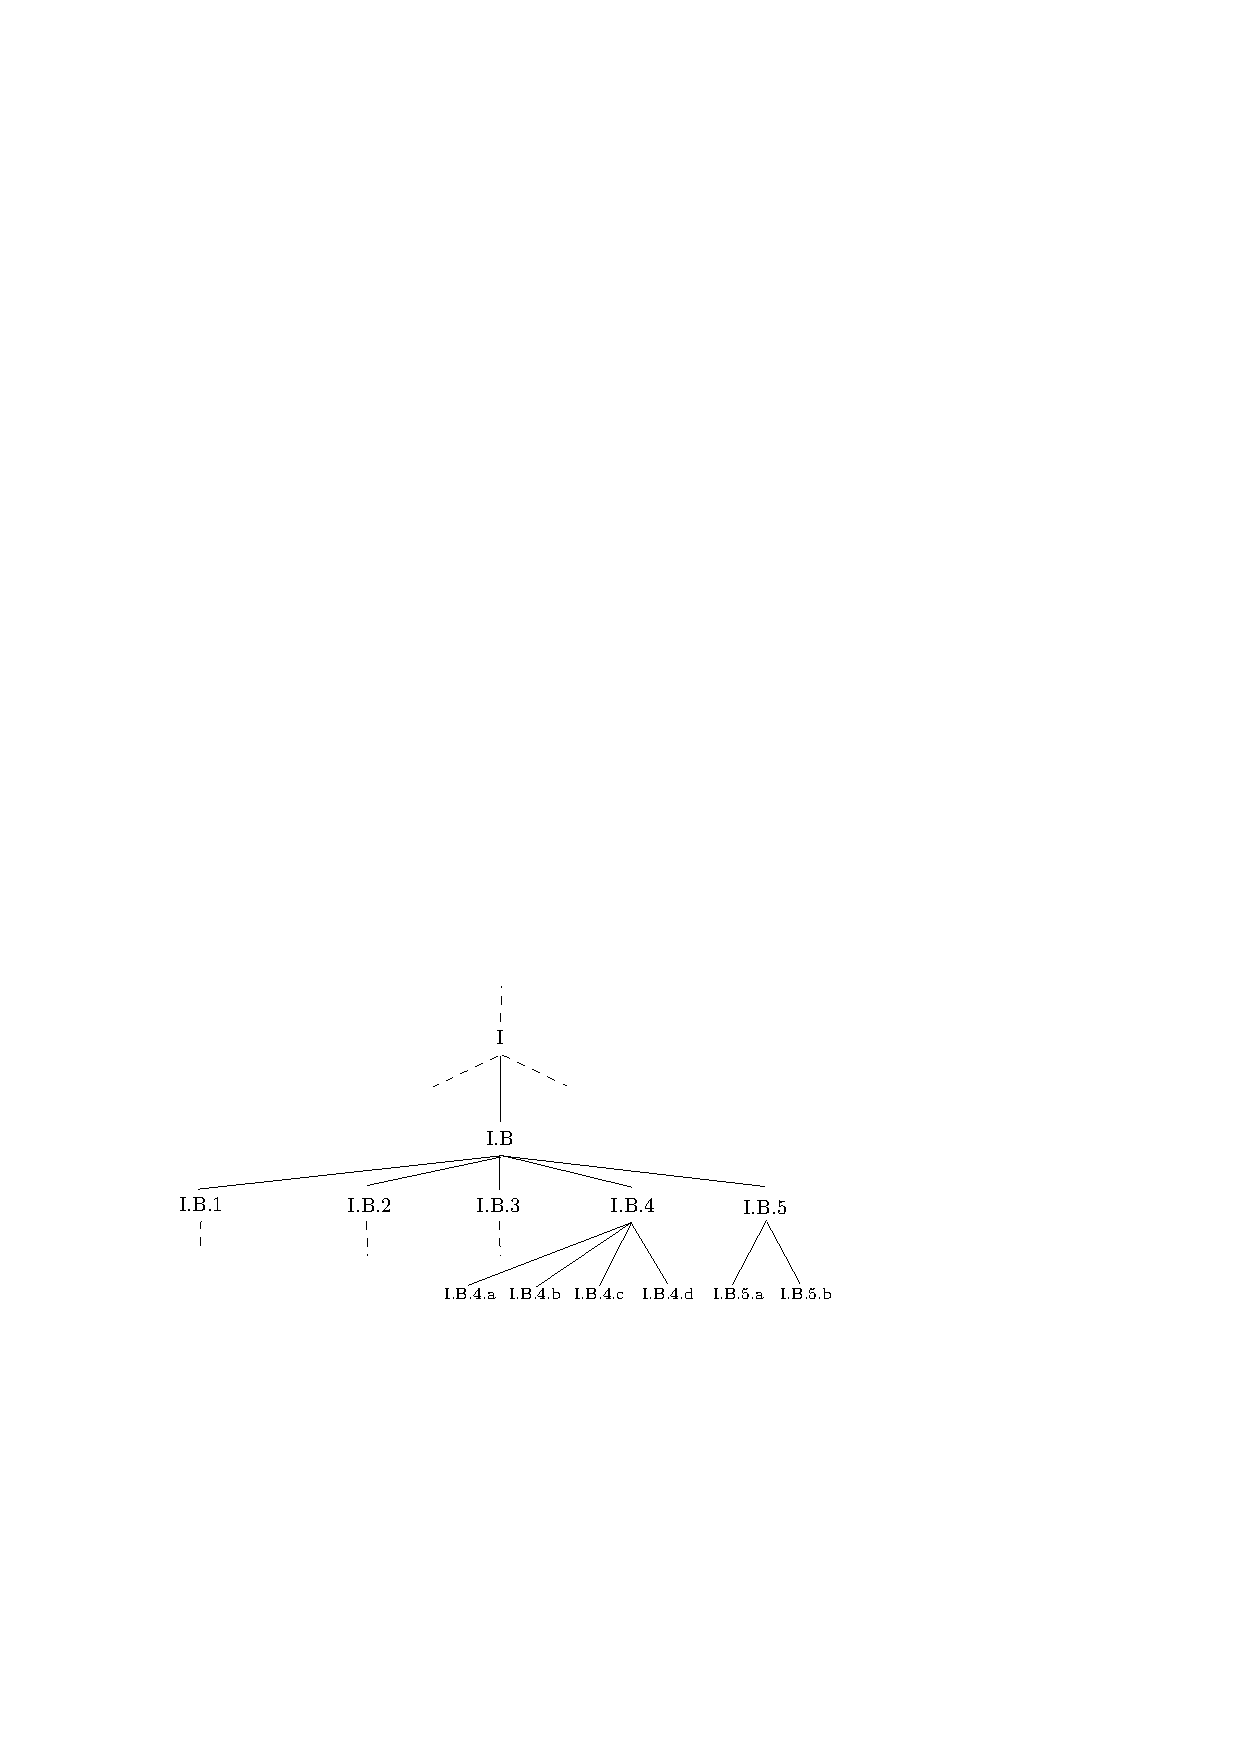
\includegraphics[width=3in]{Graphic/Pictures/ThesauTN.pdf}
 % ThesauTN.pdf: 595x842 pixel, 72dpi, 20.99x29.70 cm, bb=0 0 595 842

\vspace*{3ex}
\begin{Itabular}{llr|llr}
Non-human world & I& - & Shea & I.B.4.b & 2 \\ 
Animals and Plants & I.B &-  &  Fruit, seed & I.B.4.c &31 \\ 
Animals-wild & I.B.1 & 40&  Flower & I.B.4.d &2\\
Birds-wild &  I.B.2 & 30& Plants : plant products & I.B.5 &23 \\
Smaller-creatures & I.B.3 &107 & Leaf & I.B.5.a  & 10 \\ 
Trees &  I.B.4 & 92 & Grass & I.B.5.b & 11 \\ 
 Root & I.B.4.a & 2 & && \\
\end{Itabular} 
\end{center}

\caption[Excerpt of the Thesaurus for north-Ghanaian
Languages]{Excerpt of the Thesaurus for north-Ghanaian
Languages \citep{Nade07}\label{fig:LEX-ThesauTN}}
\end{figure}




% I.B.1: 40
% I.B.1.a: 1
% I.B.1.b: 1
% I.B.1.c: 11
% I.B.2: 30
% I.B.3: 10
% I.B.3.a: 2
% I.B.3.b: 35
% I.B.3.c: 60
% I.B.4: 92
% I.B.4.a: 2
% I.B.4.c: 31
% I.B.4.d: 2
% I.B.5: 23
% I.B.5.a: 10
% I.B.5.b: 11

%more on sem domain
 %lexicology: study of the lexical inventory and relations and structures of a language.
\clearpage


\subsubsection{Dictionary-Index abbreviations}
\label{LEX:abbrev}


\tablefirsthead{}
\tablehead{%
%\midrule
\multicolumn{2}{l}{\textit{continued from previous page}}\\
%\midrule
}
\tabletail{
%\midrule
\multicolumn{2}{r}{\textit{continued on next page}}\\
}
%\midrule
\tablelasttail{}
%\bottomcaption{ \label{tab:}}
\xentrystretch{0.15} 
 \begin{Ixtabular}{ll}
adv & adverb\\
abl & ability\\
art& article\\

clf& classifier\\
comp&complementizer\\
conn& connective\\
cpx & complex\\

dem&demontrative\\

egr &egressive\\

foc & focus\\

hum+&human\\
hum-&non-human\\


ideo & ideophone\\
idiom & idiom\\
imp & imperative\\
ingr & ingressive\\
interg& interrogative  \\
interj & interjection\\ %like gafra, greetings,...
ipfv & imperfective \\
itr & iterative\\

n & noun\\
neg & negation\\
num&numeral\\

ono&onomatopoeia\\

phr& phrase\\
 Pl &plural\\
poss & possessive\\
postp&postposition\\
pro & pronoun\\
propn&proper noun\\

qual & qualifier\\
quant&quantifier\\

reflex&reflexive   \\ % tIntIn
rel.n& relational noun\\

sg&singular\\
st&strong pronoun\\

tam& tense/aspect/mood particle\\

ultm. & ultimately\\

v&verb\\

wk&weak pronoun\\

1& first person\\
2& second person\\
3&third person\\

%%%%%%%%%%%%%%%%
Ant& antonym\\
\underline{\it Amarantus Debius} & scientific name\\
Enum& enumarative usage of a numeral\\
Etym& etymology\\
From & borrowed word\\
Lit & literal meaning\\
See &cross-reference\\
SynT&  taboo synonym\\
Usage& village where the form is used\\
Variant & variant form\\
\end{Ixtabular}


\cleardoublepage

%\begin{comment}
%\thispagestyle{empty}
%\begin{titlepage}
%\label{tit:Dic}
\begin{center}
\vspace*{1.5in}
{\huge Chakali-English Dictionary}
\par
\end{center}
%\end{titlepage}
\cleardoublepage


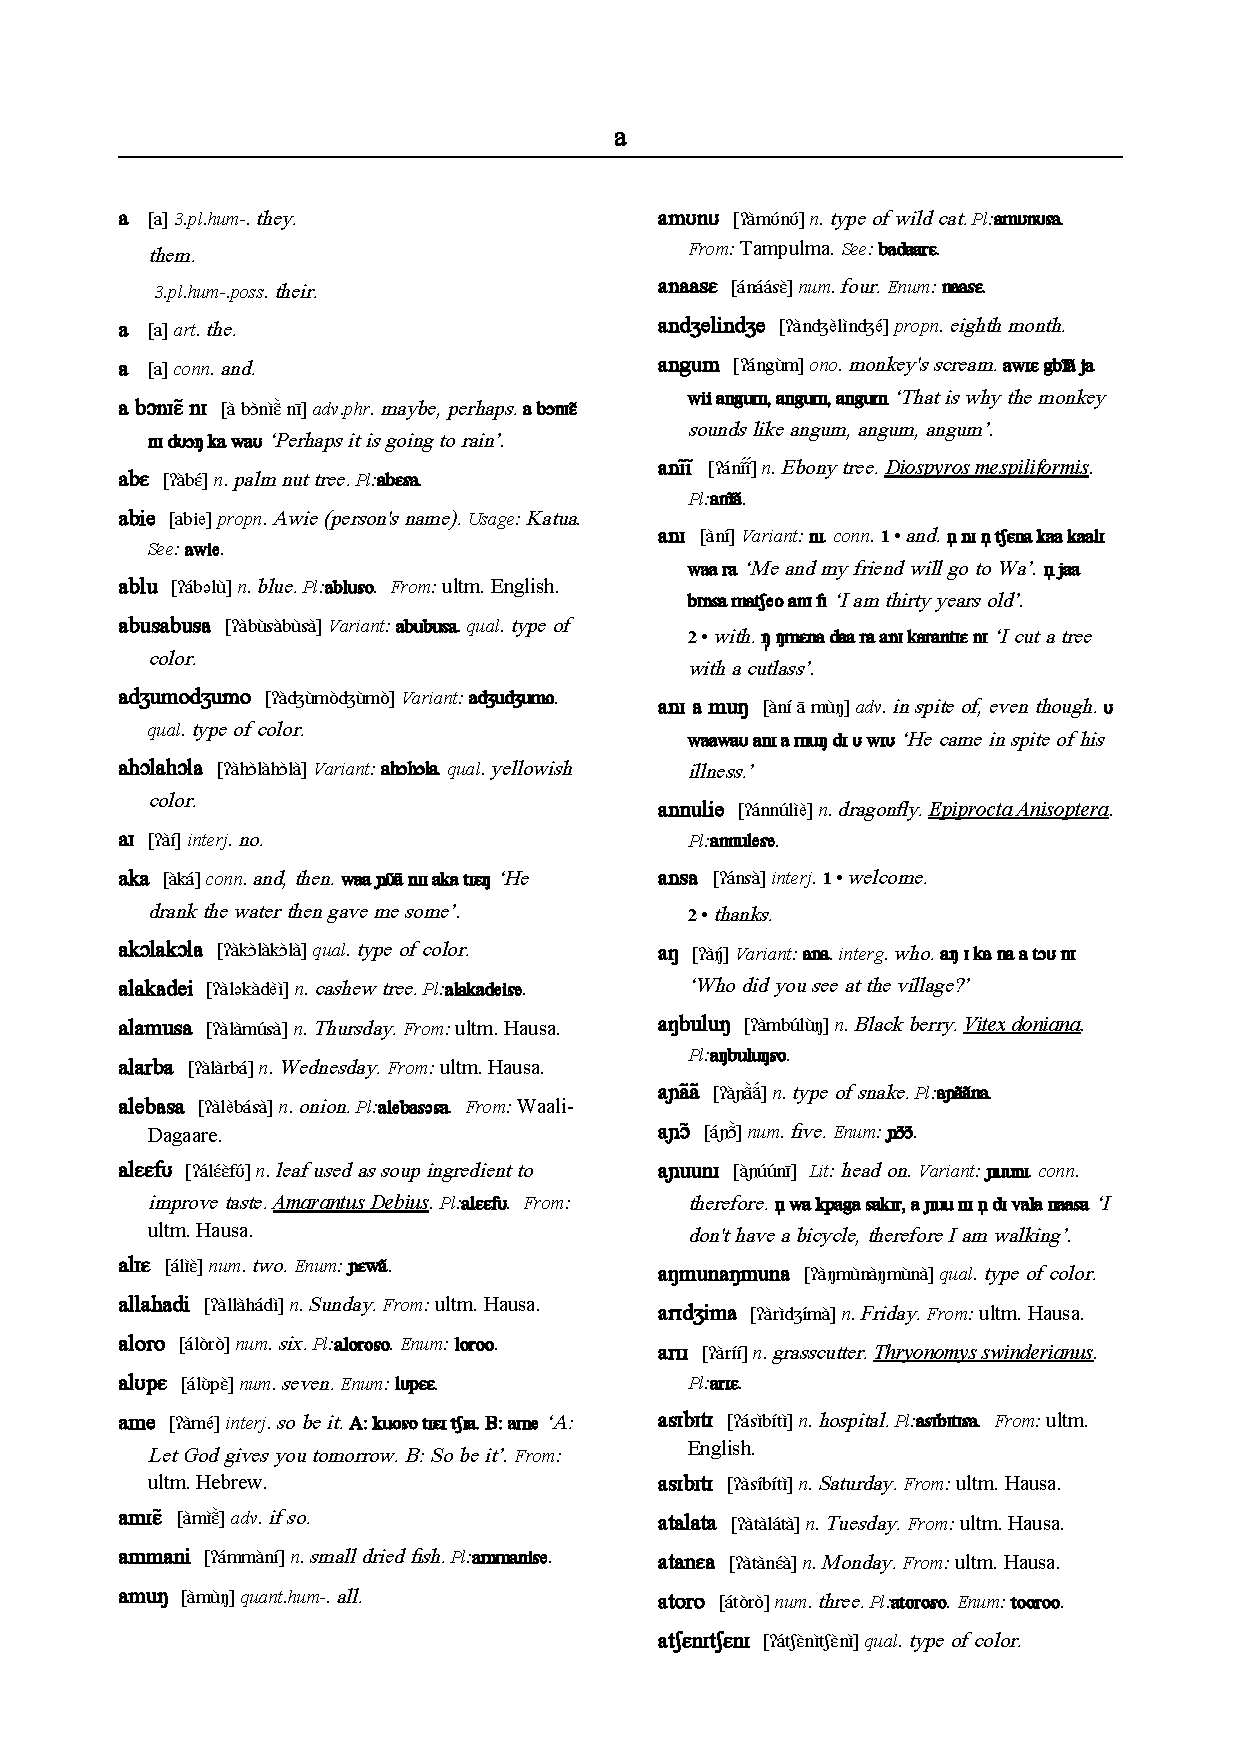
\includepdf[pages=- , offset=-5mm -5mm, scale=.8,
pagecommand={}]{Graphic/Pictures/dic018.pdf}


\cleardoublepage

%\thispagestyle{empty}

%\begin{titlepage}

\begin{center}
\vspace*{1.5in}
{\huge English-Chakali Index}
\par
\end{center}
%\end{titlepage}
 %\vspace*{0.5in}

% \pagebreak
\cleardoublepage


 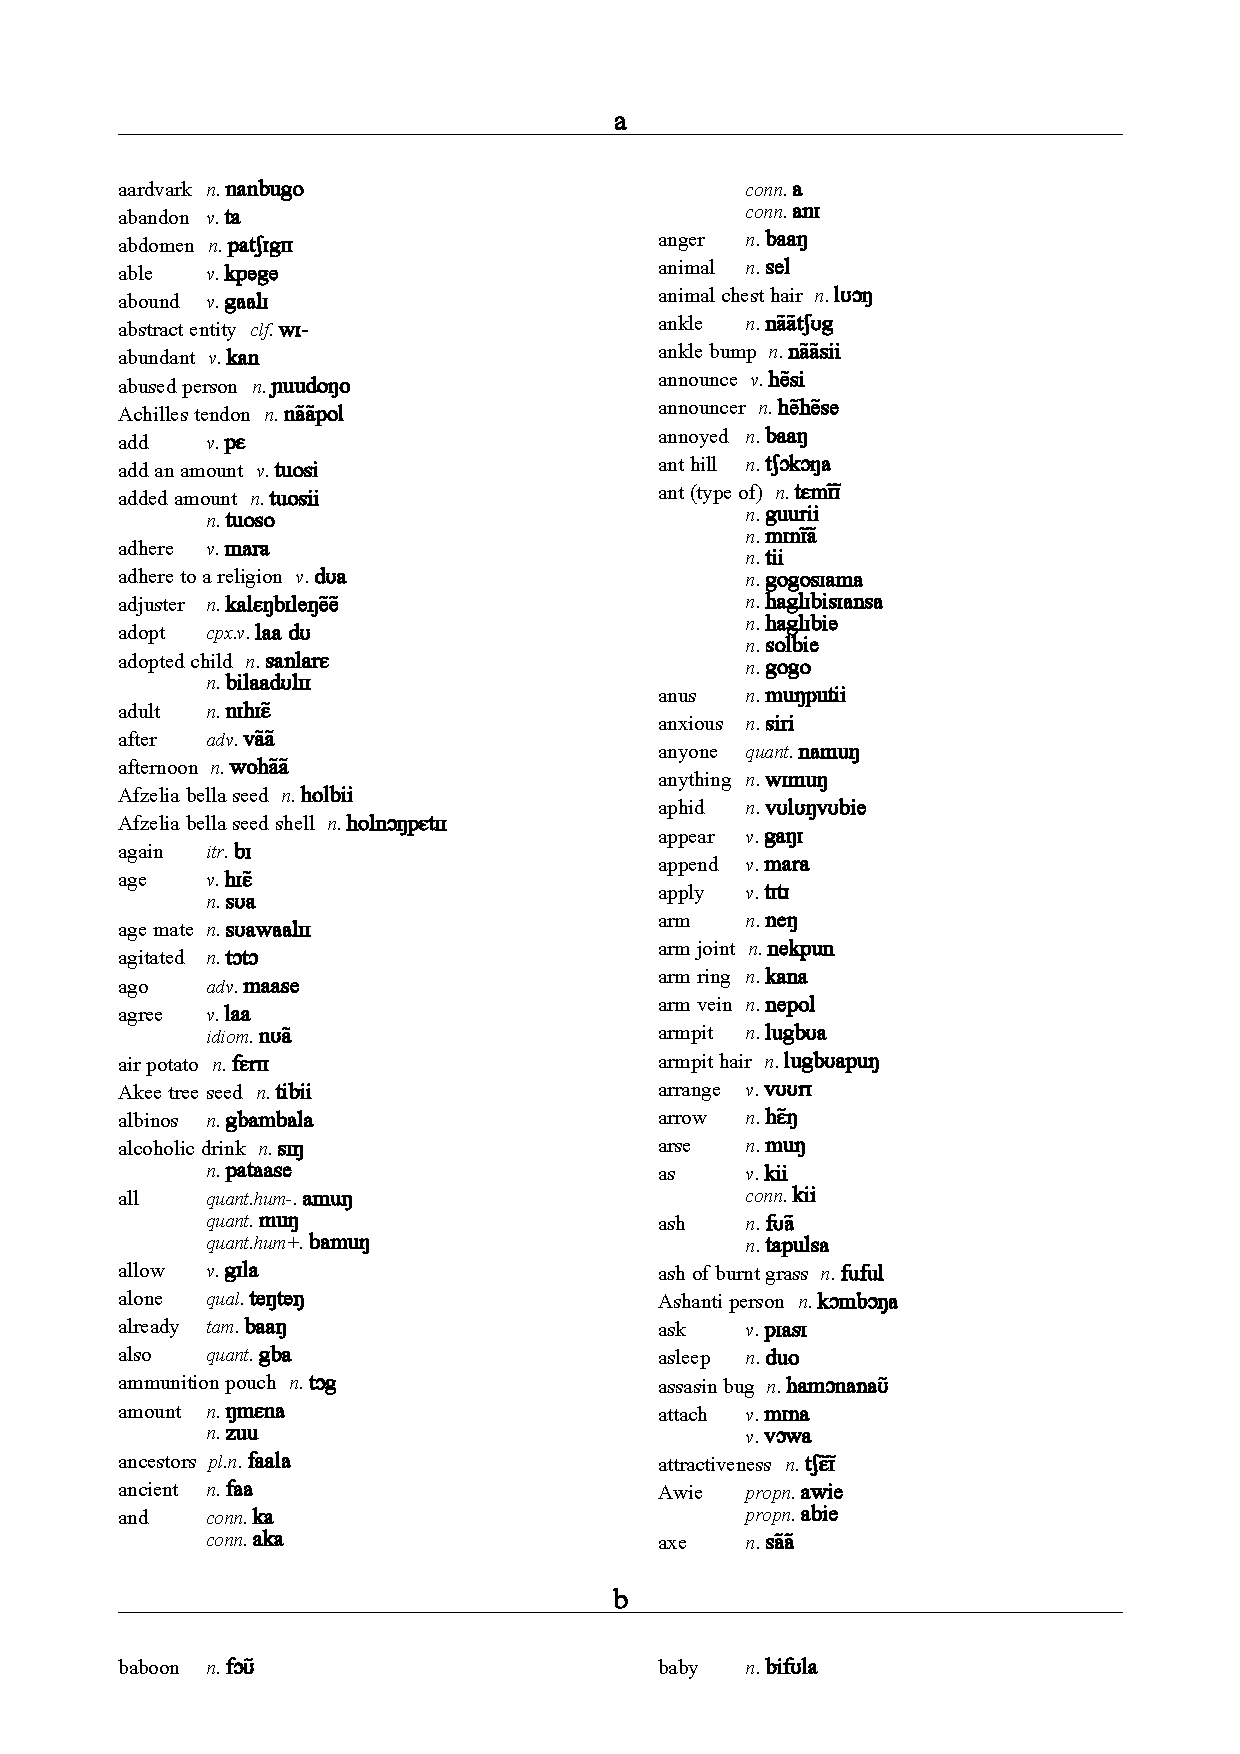
\includepdf[pages=- , scale=.8, offset=-5mm -5mm, pagecommand={}
]{Graphic/Pictures/index018.pdf}


%pagecommand= \pagestyle{fancy}

%\end{comment}
